\begin{frame}
  \frametitle{First year optics: A simple optical fibre}

  Step index optical fibre utilizing total internal reflection
  \begin{itemize}
  \item core of material with refractive index $n_1$
  \item outer shell of material with refractive index $n_2 < n_1$
  \end{itemize}
  Acceptance angle is $\sin\theta\idx{max} = \sqrt{n_1^2 - n_2^2}$
  when assuming $n=1$ outside the fibre.

  \begin{center}
    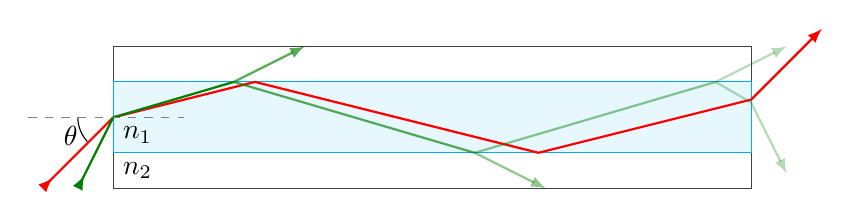
\begin{tikzpicture}[scale=0.9]
      \draw[thin,black!75] (2,-1) rectangle +(9,2);
      \fill[cyan!10,draw=cyan,thin] (2,-.5) rectangle +(9,1);
      \draw[thick,red,latex reversed-latex]
        (1,-1) -- (2,0) -- ++(2,.5) -- ++(4,-1) -- ++(3,.75) -- ++(1,1);
        \begin{scope}[green!50!black,thick]
        \draw[thick,latex reversed-]
          (1.5,-1) -- (2,0) -- (3.7,.5);
        \draw[thick,opacity=.66] (3.7,.5) -- (7.1,-.5);
        \draw[thick,opacity=.66,-latex] (3.7,.5) -- +(1,.5);
        \draw[thick,opacity=.44] (7.1,-.5) -- (10.5,.5); 
        \draw[thick,opacity=.44,-latex] (7.1,-.5) -- +(1,-.5);
        \draw[thick,opacity=.29,-latex] (10.5,.5) -- (11,.21) -- +(.5,-1);
        \draw[thick,opacity=.29,-latex] (10.5,.5) -- +(1,.5);
      \end{scope}
  
      \node[anchor=south west] at (2,-.5) {$n_1$};
      \node[anchor=north west] at (2,-.5) {$n_2$};
      
      \draw[thin,dashed,gray] (.8,0) -- (3,0);
      % node[above,at start,anchor=south west] {Normal};
      \draw[thin] (1.5,0) arc (180:223:.5)
      node[left,anchor=east,yshift=2pt] {$\theta$};
    \end{tikzpicture}
  \end{center}

  Trivially, rays with angle of incidence greater than the acceptance
  angle of the fibre will be lost.
\end{frame}


\begin{frame}
  \frametitle{Better fibres: Graded-index}

  Graded-index fibre (wide industrial usage)
  \begin{itemize}
  \item refractive index varies radially, maximal at the center
  \item does not rely on total internal reflection
  \end{itemize}
  Rays are gradually refracted towards the axis, where the refraction
  index is maximal. Here too, the fibre has a certain acceptance.

  \begin{center}
    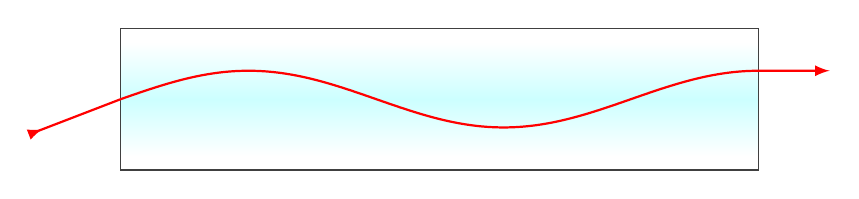
\begin{tikzpicture}[scale=0.9]
      \shade[top color=white,bottom color=white,middle color=cyan!20]
        (2,-.8) rectangle +(9,1.6);
      \draw[thin,black!75] (2,-1) rectangle +(9,2);
      \draw[thick,red,latex reversed-latex] (.7,-.5) -- (2,0) sin (3.8,.4)
       cos (5.6,0) sin (7.4,-.4) cos (9.2,0) sin (11,.4) -- +(1,0);
      % \fill[cyan!10,draw=cyan,thin] (2,-.5) rectangle +(9,1);
      % \draw[thick,red,latex reversed-latex]
      %   (1,-1) -- (2,0) -- ++(2,.5) -- ++(4,-1) -- ++(3,.75) -- ++(1,1);
      %   \begin{scope}[green!50!black,thick]
      %   \draw[thick,latex reversed-]
      %     (1.5,-1) -- (2,0) -- (3.7,.5);
      %   \draw[thick,opacity=.66] (3.7,.5) -- (7.1,-.5);
      %   \draw[thick,opacity=.66,-latex] (3.7,.5) -- +(1,.5);
      %   \draw[thick,opacity=.44] (7.1,-.5) -- (10.5,.5); 
      %   \draw[thick,opacity=.44,-latex] (7.1,-.5) -- +(1,-.5);
      %   \draw[thick,opacity=.29,-latex] (10.5,.5) -- (11,.21) -- +(.5,-1);
      %   \draw[thick,opacity=.29,-latex] (10.5,.5) -- +(1,.5);
      % \end{scope}
  
      % \node[anchor=south west] at (2,-.5) {$n_1$};
      % \node[anchor=north west] at (2,-.5) {$n_2$};
      
      % \draw[thin,dashed,gray] (.8,0) -- (3,0);
      % % node[above,at start,anchor=south west] {Normal};
      % \draw[thin] (1.5,0) arc (180:223:.5)
      % node[left,anchor=east,yshift=2pt] {$\theta$};
    \end{tikzpicture}
  \end{center}
  For a parabolic index profile rays follow sinusoidal paths, with
  paths and acceptances generally determined by the index profile and
  beam intensity profile.

\end{frame}


\begin{frame}
  \frametitle{Qualitative description of the Kerr effect}

  \begin{itemize}
  \item In an optical fibre, the refractive index i fixed upon
    manufacture. Conversely, the refractive index in a Kerr-medium is
    \alert{induced} by the electrical field of the propagating laser.

  \item The qualitative description of the propagating light is
    similar, as individual rays sees an effective refractive index
    depending on the rays particilar value of the electric field.

  \item For gaussian beams, the electric field depends on the distance
    from the beam axis and beam waist. Hence, the effective refractive
    index varies for certain parts of the beam.
  \end{itemize}
\end{frame}


\begin{frame}
  \frametitle{Self-focusing}

  \begin{itemize}
  \item Self-focusing takes place when the induced refractive index is
    sufficiently high, ie. for beams and parts thereof with high
    intensity.

  \item At low intensity the induced refractive index is insufficient
    to overcome diffractive spreading. At very high intensity the
    materiale breaks down.

  \item For a gaussian beam inverse focal length (dioptic power) is
    determined by the beam parameters and the nonlinear component of
    the refractive index of the Kerr-medium
    \begin{align*}
        f\idx{kerr}\inv = \frac{4}{\pi} \frac{n_2 P}{w_0^4} z,
    \end{align*}
    where $z$ is the distance traveled in the medium.

  \item Major advantage: Optical axis is induced by the beam.
  \end{itemize}

\end{frame}


%%% Local Variables: 
%%% mode: latex
%%% TeX-master: "nonlinearslides"
%%% End: 
